%% ============================================================
%% The Researcher-Agent Problem: A Principal-Hierarchy Framework
%% for AI-Assisted Knowledge Production in Public Administration
%%
%% Target: Public Administration Review
%% Authors: Edmund Poku Adu, PhD
%%          Arkansas State University
%% Session: PA_20260227_1400
%% ============================================================

\documentclass[12pt]{article}

%% --- Packages ---
\usepackage[margin=1in]{geometry}
\usepackage{setspace}
\doublespacing
\usepackage{times}
\usepackage[round,sort&compress]{natbib}
\usepackage{booktabs}
\usepackage{threeparttable}
\usepackage{array}
\usepackage{hyperref}
\hypersetup{colorlinks=true, linkcolor=black, citecolor=black, urlcolor=black}
\usepackage{graphicx}
\usepackage{caption}
\usepackage{tabularx}
\usepackage{amsmath}
\usepackage{amssymb}
\usepackage{pifont}
\usepackage{tikz}
\usetikzlibrary{arrows.meta, positioning, shapes.geometric, calc, decorations.pathreplacing, fit, backgrounds}
\usepackage{float}

%% PAR: blind review
\title{\textbf{The Researcher-Agent Problem: \\
A Principal-Hierarchy Framework for AI-Assisted \\
Knowledge Production in Public Administration}}

\date{}
\author{}   % blind

\begin{document}

\maketitle
\thispagestyle{empty}

% -------------------------------------------------------
%  ABSTRACT
% -------------------------------------------------------
\begin{abstract}
\noindent
Artificial intelligence agents now assist researchers across the full arc of scholarly
production, yet public administration lacks a theoretical framework governing this
cognitive delegation. This article develops the \emph{Research-Agent Principal Hierarchy}
(RAPH): a three-tier governance model in which field institutions serve as meta-principal,
the researcher serves as principal, and the AI system serves as agent. The framework
identifies three agency problems (information asymmetry, moral hazard, adverse selection)
and derives four testable propositions. A single instrumental case study of a complete
AI-assisted manuscript production pipeline, documented through verbatim session logs,
tests these propositions across a 10-stage research workflow. The case supports all four
propositions, identifies a previously untheorized ``double-hazard'' condition at
high-complexity, low-reversibility stages, and reveals that tiered monitoring protocols
fail at exactly the junctures where they matter most. The article concludes with
structurally enforced commitment gates and calls on journals, IRBs, and ASPA to develop
governance standards for AI-assisted scholarship.

\bigskip
\noindent\textbf{Keywords:} artificial intelligence, principal-agent theory, research governance,
agentic AI, knowledge production, methodological equity, public administration scholarship
\end{abstract}

\newpage

\bigskip
\noindent\textbf{Practitioner Points}
\begin{itemize}\setlength{\itemsep}{2pt}
  \item AI agents now assist PA researchers across the full pipeline, creating governance
    gaps. The RAPH framework shows that information asymmetry, moral hazard, and adverse
    selection arise predictably in AI-assisted workflows.
  \item AI-assisted research with preserved interaction logs is \emph{more} transparent and
    \emph{more} accountable than traditional research with no audit trail. Documented
    workflows enable detection of p-hacking, HARKing, and selective reporting.
  \item The reviewer pool must expand to match accelerating manuscript production. The
    Jethro Principle distributes review tasks across bachelor's, master's, and doctoral
    students with structured rubrics, reserving expert judgment for high-stakes evaluations.
  \item PA journals must eliminate opaque rejection, adopt AI-workflow disclosure standards,
    and permit transparent AI-assisted reviewing --- leading by example with the democratic
    governance principles the field studies.
  \item Under-resourced PA researchers face the highest governance burden; journals
    and ASPA through the Jethro framework can create shared audit infrastructure and technical review support.
\end{itemize}

\newpage


% -------------------------------------------------------
%  1. INTRODUCTION
% -------------------------------------------------------
\section{Introduction}

Public administration's engagement with artificial intelligence has been almost entirely
outward-facing. The field asks how AI reshapes government service delivery
\citep{zhu2025public, oecd2025governing}, how algorithmic systems alter bureaucratic
discretion \citep{bullock2019artificial, buffat2015street}, and how public organizations
should be held accountable when automated decisions harm citizens
\citep{diakopoulos2016accountability, meijer2021algorithmicbureaucracy}. These questions
matter. But a different AI adoption is occurring simultaneously, inside the scholarly
enterprise itself, and the field has not noticed.

Artificial intelligence agents now assist researchers across the entire arc of manuscript
production. They retrieve and synthesize literatures \citep{schmidgall2025agent},
generate and evaluate theoretical frameworks, write and debug statistical code, and draft
journal-quality prose. Tools purpose-built for social science research (such as Elicit,
ResearchAgent, and Agent Laboratory) can reduce systematic review screening by more than 60
percent while maintaining recall above 90 percent \citep{hasan2024integrating}. What once
required a team of graduate research assistants can now be executed by a single researcher
with an AI system and a well-designed workflow.

This development raises governance questions that public administration is better equipped
than any other social science to answer. The field's foundational theoretical infrastructure
(principal-agent theory, accountability frameworks, bureaucratic governance) was built
precisely to analyze what happens when cognitive work is delegated across organizational
hierarchies and how accountability is preserved when principals cannot fully observe agents.
Those tools apply with considerable precision to the researcher-AI relationship. Yet no one
has applied them.

This article develops the \emph{Research-Agent Principal Hierarchy}
(RAPH), a three-tier framework in which field institutions (journals, IRBs, professional
norms) govern researchers, who in turn delegate cognitive research tasks to AI agents, and
theorizes the agency problems that arise at each tier. The article tests the framework against a
documented case: a complete 10-stage AI-assisted manuscript production pipeline conducted
by a solo researcher at a regional teaching university, with every researcher-agent
interaction recorded in verbatim session logs and structured workflow state files. The case
is not a thought experiment: it is the research process that produced this article,
documented as it occurred.

The RAPH framework gives public administration a theoretical vocabulary for governing
AI-assisted research that did not previously exist. The case reveals a ``double-hazard''
condition at framework and analysis stages, where high cognitive complexity coincides with
low decision reversibility, moral hazard peaks, and monitoring is least likely to occur.
The case also demonstrates that tiered governance protocols fail at these junctures when left
to researcher discretion, and that structurally enforced commitment gates must replace
voluntary protocols. These findings carry direct implications for journal editors, IRBs,
professional associations, and the growing population of researchers who use AI agents in
their work.

% -------------------------------------------------------
%  2. LITERATURE REVIEW
% -------------------------------------------------------
\section{AI in Public Administration: From Government Tools to Research Tools}

\subsection{The Outward-Facing Literature}

Public administration's AI scholarship has developed three interrelated themes. The first is
algorithmic governance: how AI-driven decision systems in government change the nature of
administrative action, the distribution of public services, and the accountability structures
that constrain them \citep{meijer2021algorithmicbureaucracy, diakopoulos2016accountability,
sun2023algorithmicdiscrimination}. The second is AI and bureaucratic discretion: building on
\citeauthor{lipsky1980street}'s \citeyearpar{lipsky1980street} foundational account of
street-level workers, scholars have examined how AI systems alter the discretionary space
of frontline bureaucrats \citep{bullock2019artificial, buffat2015street, evans2004streetlevel}.
The third is human-AI interaction in public sector decisions: how automation bias, skeuomorphism,
and cognitive off-loading reshape the judgments of public managers who work alongside AI
systems \citep{alon2023human, engstrom2020govtautomation}.

Across these three themes, the referent actor is the government: the agency deploying AI,
the bureaucrat operating alongside it, the citizen receiving its outputs. The public
administration researcher appears nowhere in this literature as a subject of theoretical
attention.

\subsection{The AI Research Workflow Revolution}

This inattention is consequential, because the tools available to researchers have undergone
a rapid transformation. Large language models with agentic capabilities now execute multi-step
research tasks with minimal human instruction \citep{gridach2025agenticscientific,
hasan2024integrating}. Systems like Agent Laboratory \citep{schmidgall2025agent}
can conduct literature searches, generate hypotheses, write and execute code, and produce
draft manuscripts. \citet{lehr2024chatgpt} show that ChatGPT already performs
competently as a research librarian and research ethicist, detecting methodological violations
and assessing replication failures.

The implications for research governance have not been ignored outside public administration.
\citet{elephantinthelab2025reproducibility} document how AI-assisted research creates a
reproducibility crisis: when reasoning steps are not logged, replication becomes ``a lottery.''
\citet{oecd2025governing} note that 33 percent of governments already use AI in policy
functions, but systematic governance frameworks for AI-assisted knowledge production remain
absent across the social sciences.

\subsection{The Governance Gap}

Public administration has the theoretical infrastructure to address this gap. Principal-agent
theory, developed in economics \citep{jensen1976theory} and adapted for public administration
by \citet{mitnick1973politicaleconomy}, \citet{moe1984neweconomics}, and \citet{waterman1998agents},
provides a mature framework for analyzing exactly the governance problem that AI-assisted
research creates: a principal who delegates cognitive work to an agent, cannot fully observe
the agent's effort, and faces accountability to a higher-level authority for the outputs. The
question is not whether this framework applies (it manifestly does) but how it must be
specified for the research context.

Three aspects of the research-agent relationship distinguish it from the standard governmental
principal-agent problem. The agent here is not a human bureaucrat but a computational system
whose ``effort'' takes the form of probabilistic token generation, a different information
asymmetry structure than the conventional case. The principal (the researcher) is simultaneously
the producer of the output and the primary monitor of the agent; there is no separation of
production and oversight analogous to the legislative-bureaucratic split. And the meta-principal
(the field, journals, IRBs) currently lacks the governance instruments to audit AI-assisted
research, creating a vacuum that the framework developed below aims to fill.

% -------------------------------------------------------
%  3. THEORETICAL FRAMEWORK
% -------------------------------------------------------
\section{The Research-Agent Principal Hierarchy}

\subsection{Three-Tier Architecture}

The Research-Agent Principal Hierarchy (RAPH) organizes the governance relationships in
AI-assisted scholarship into three tiers, each with distinct roles, interests, and
accountability relationships.

\textbf{Tier 1 --- Meta-Principal: The Field and Its Institutions.}
Academic journals, institutional review boards, professional associations (in public
administration, the American Society for Public Administration), and the informal norms of
the scholarly community constitute the meta-principal. The meta-principal sets governance
standards for what counts as credible knowledge and how it must be produced and reported.
It monitors researcher-principals not through direct observation of the research process but
through the outputs submitted for publication: manuscripts, data, code, and replication
materials. In the conventional research relationship, this monitoring is sufficient because
the researcher is also the primary producer of all outputs, and the chain of accountability
is short. AI-assisted research breaks this assumption: outputs are co-produced by an agent
whose contributions may not be attributable or auditable under current reporting norms.

\textbf{Tier 2 --- Principal: The Researcher.}
The researcher is the central actor in the hierarchy, simultaneously subordinate to the
meta-principal's governance authority and superior to the AI agent's delegated work. The
researcher makes delegation decisions (which tasks to assign to the agent, which to retain)
and bears full accountability to the meta-principal for all outputs, regardless of their
origin in the researcher-agent workflow. This accountability gap is the fundamental governance
problem of AI-assisted research: the principal bears costs (reputational, professional) for
agent errors that she may not have sufficient information or capacity to prevent.

\textbf{Tier 3 --- Agent: The AI Research System.}
The AI agent executes delegated tasks (searching literature, generating code, building
theoretical frameworks, drafting text) and returns outputs to the researcher for evaluation
and integration. Unlike a human research assistant, the agent's ``reasoning'' is not
transparent to the researcher; it cannot explain why a particular synthesis, argument,
or statistical specification was preferred. This opacity is the structural source of
information asymmetry in the RAPH.

\subsection{Three Agency Problems}

Drawing on the canonical treatments of \citet{jensen1976theory} and \citet{waterman1998agents},
the RAPH identifies three agency problems that arise in the hierarchy.

\textbf{Information Asymmetry.}
The researcher-principal cannot observe the AI agent's inferential process: the reasoning
steps, source weightings, and probabilistic choices that produce a given output. This
asymmetry is not constant across the research workflow; it scales with the cognitive
complexity of the delegated task. For low-complexity tasks (keyword search, table formatting),
the output is easily verified against observable criteria. For high-complexity tasks
(theoretical framework development, causal interpretation, literature synthesis of contested
debates), the output requires expertise-intensive evaluation that may exceed the researcher's
available time and attention. The asymmetry peaks at exactly the tasks where the agent's
contribution is most consequential for the credibility of the research product.

\textbf{Moral Hazard.}
Once the researcher delegates a high-cognitive-cost task to the agent, the marginal benefit
of monitoring the output decreases relative to the monitoring cost. The researcher who has
delegated literature synthesis to an agent has saved time; investing that saved time in
exhaustive verification erases the efficiency gain. This creates a structural incentive to
under-monitor, which is classical moral hazard \citep{holmstrom1979moral}. Moral hazard,
however, is not uniform across the workflow; it is moderated by task reversibility.
At high-reversibility stages (early search, initial framework exploration), under-monitoring
carries low expected cost because errors can be corrected cheaply. At low-reversibility
stages (framework commitment, statistical specification, final causal interpretation),
under-monitoring is catastrophically expensive because errors propagate forward through
all subsequent stages. Moral hazard thus peaks at exactly the junctures where its cost is
greatest.

\textbf{Adverse Selection.}
The governance burden of AI-assisted research falls differentially across the researcher
population. Researchers at well-resourced institutions with dedicated graduate students,
senior co-authors, and specialist collaborators have institutional infrastructure that
functions as distributed monitoring: errors that escape individual attention are caught by
the team. Researchers at teaching-focused institutions with minimal research infrastructure
lack these redundant oversight layers. Yet the latter group faces the same (or greater)
incentive to use AI agents to compensate for resource limitations. The result is an adverse
selection structure: the researchers most likely to adopt AI agents for resource-compensating
reasons are those least equipped to govern them effectively, concentrating governance failures
where research infrastructure is already thin.

\subsection{Four Theoretical Propositions}

From the RAPH and its three agency problems, the article derives four theoretical propositions to be
tested against the case evidence.

\textbf{P1 (Information Asymmetry Gradient):} As the cognitive complexity of a delegated
research task increases, the information asymmetry between researcher-principal and AI agent
increases, raising the probability of undetected inferential error proportionally. Zero
researcher overrides at high-complexity stages reflect asymmetry-consistent acceptance, not
adequate monitoring.

\textbf{P2 (Moral Hazard at Commitment Junctures):} Researcher-principals systematically
under-monitor AI agent outputs when task reversibility is low, because the monitoring cost
exceeds the expected cost of undetected error as evaluated at the time of delegation. Moral
hazard is most acute at double-hazard junctures where low reversibility coincides with
high cognitive complexity.

\textbf{P3 (Adverse Selection and Methodological Inequality):} The governance burden of
AI-assisted research falls disproportionately on researchers at resource-constrained
institutions, producing a regressive distributional effect in which AI agent adoption
amplifies rather than attenuates existing methodological inequality.

\textbf{P4 (Conditional Sufficiency of Tiered Monitoring):} A governance framework that
calibrates researcher oversight intensity to the combined function of task cognitive complexity
and task reversibility can reduce agency costs without eliminating efficiency gains, but
only when commitment gates at double-hazard junctures are structurally enforced rather than
left to researcher discretion.

\bigskip

[Figure 1 here]

\bigskip

% -------------------------------------------------------
%  4. METHOD
% -------------------------------------------------------
\section{Method}

\subsection{Case Study Design}

The analysis employs a single instrumental case study \citep{stake1995art, yin2014case}. The case
(a complete AI-assisted manuscript production pipeline executed by a solo researcher at a
regional teaching university) is studied not for its intrinsic interest but as an instrument
for testing the RAPH's theoretical propositions. Three rationales support single-case design
\citep{yin2014case}: the case is a \emph{critical} case that satisfies all conditions
specified by the theoretical framework; it is an \emph{extreme} case occupying the
adverse-selection boundary predicted by P3; and it is a \emph{revelatory} case providing
access to evidence (complete verbatim researcher-agent interaction logs) not previously
available in this research domain.

The unit of analysis is the \emph{workflow stage}: a discrete phase of the research
pipeline with a defined delegation event (researcher assigns task to agent), an agent
output, and a researcher response (accept, override, or iterate). The 10-stage pipeline
generates 10 within-case observations for pattern matching.

One feature of this design warrants explicit methodological acknowledgment: the article
being written is the same article whose production the case documents. This self-referential
structure is a strength, not a limitation. Evidence is contemporaneous rather than
retrospective; the session logs record delegation events as they occurred, not as the
researcher later recalls them. The researcher-as-subject problem, typically the deepest
vulnerability in self-study research, is mitigated precisely because the primary evidence
stream (the verbatim session transcript) lies outside the researcher's retrospective
editorial control. A researcher reconstructing past decisions from memory is susceptible
to self-serving recall; a researcher whose decisions were logged in real time is not.

\subsection{Evidence Sources}

The case draws on four documentary evidence streams.

\textit{Session transcripts} constitute the primary evidence source: complete verbatim logs
of every researcher-agent interaction from the Claude Code environment, capturing every
task delegation, agent output, and researcher response in real time. Unlike retrospective
interviews or researcher recollections, these logs are contemporaneous records not subject
to memory or self-presentation bias.

\textit{Workflow state files} provide structured records of stage-completion decisions,
framework choices, and commitment-point resolutions as time-stamped JSON files created at
each stage transition. These document the formal architecture of delegation decisions
independent of the conversational record.

\textit{Output artifacts} (literature synthesis, theoretical framework memos, proposition
statements, methodology specifications, and manuscript drafts) constitute the downstream
consequences of researcher-agent interaction. They permit verification that accepted agent
outputs were incorporated without distortion and that monitoring gaps did not propagate
errors into the research product.

\textit{Researcher memos} provide reflexivity documentation: brief structured records written
prospectively at each stage specifying what tasks were delegated, what verification was
performed, and where monitoring gaps were acknowledged. These serve as the explicit
reflexivity mechanism addressing the researcher-as-subject limitation.

\subsection{Analytic Strategy}

The analytic strategy is \emph{pattern matching} \citep{yin2014case}: case evidence coded
for observable patterns is compared to patterns predicted by each proposition. Each of the
10 workflow stages is coded on five dimensions: task complexity tier (Low / Medium / High),
task reversibility (High / Medium / Low), researcher response type (Accept / Override /
Iterate), error-detection events (present / absent), and monitoring cost (Low / Medium / High).
A structured 10-row evidence matrix organizes the coded observations.

Where observed patterns diverge from predictions, explanation building \citep{yin2014case}
traces the causal mechanism producing the divergence and evaluates rival explanations against
the documentary record before revising the theoretical framework in Stage~9.

\bigskip

[Figure 2 here]

\bigskip

\subsection{Generalizability and Limitations}

The case supports \emph{analytic generalization} \citep{yin2014case}: findings generalize
to theory, not to a population of researchers or workflows. Five limitations bound the
analysis.

First, single-case design precludes statistical generalization; the findings are
theoretical, not population-representative. Second, the researcher-as-subject creates
reflexivity risk, mitigated by contemporaneous documentary evidence not under retrospective
editorial control. Third, the case involves a single agent platform (Claude, Anthropic);
agency problem profiles may differ across architectures. Fourth, the workflow covers
manuscript production; other research tasks (fieldwork, experimental administration) may
involve different agency problem configurations. Fifth, the framework is calibrated to
2025--2026 agent capabilities and will require updating as agent autonomy increases.

% -------------------------------------------------------
%  5. FINDINGS
% -------------------------------------------------------
\section{Findings: Pattern Matching Against the RAPH Propositions}

\subsection{Evidence Matrix Overview}

table~1 presents the 10-row evidence matrix organized by workflow stage. Complexity and
reversibility are assigned based on the cognitive demands documented in the session
transcripts and the downstream commitment structure of each stage decision. Researcher
response type is coded directly from the session log. The matrix reveals the governance
landscape of the AI-assisted research pipeline: a terrain of low-stakes efficient delegation
at early stages, interrupted by acute governance failures at the theoretically predicted
double-hazard junctures.

\bigskip

[Table 1 here]

\bigskip

\bigskip

[Figure 3 here]

\bigskip

\subsection{P1: Information Asymmetry Gradient}

The case supports P1 at all 10 stages. The evidence reveals a consistent asymmetry gradient
aligned with task complexity: at Stages 1--2 (literature search, journal profiling), agent
outputs were factual and verifiable, information asymmetry was low, and researcher acceptance
reflected appropriate trust rather than monitoring failure. At Stages 4--5 (theoretical
framework development, proposition derivation), agent outputs encoded theoretical assumptions
(which canon to cite, what the framework's boundary conditions are, how the propositions
connect to governance prescriptions) that were accepted without interrogation.

The case refines P1 in an important respect. Zero override events at high-complexity
stages are \emph{not} equivalent to zero override events at low-complexity stages, even
though they produce identical data records. At Stage 4, the researcher responded to a
2,000-word theoretical framework exposition with a single-character acceptance. This is not
the behavior of a researcher who evaluated the framework and found no errors; it is the
behavior of a researcher whose monitoring capacity was exceeded by the asymmetry. The
governance implication is that monitoring sufficiency cannot be inferred from the absence
of overrides; it must be inferred from documented monitoring procedures. A researcher who
records ``reviewed framework against Waterman \& Meier (1998), verified that the
three-tier hierarchy is consistent with Moe's (1984) legislative-bureaucratic principal
structure, and confirmed that P1--P4 follow logically from the asymmetry-moral hazard-adverse
selection sequence'' has engaged in monitoring. A researcher who records ``1'' has not.

\subsection{P2: Moral Hazard at Commitment Junctures}

P2 receives its strongest support from Stage 4, which produced the case's most striking
evidentiary moment. The agent had delivered a 2,189-word output: three fully elaborated
theoretical frameworks (Research-Agent Principal Hierarchy, Inferential Discretion Theory,
and Competing Institutional Logics), each with a canonical literature review, a core
argument stated in three tiers, a governance prescription, a statement of PAR fit, and a
risk profile. The comparison table alone ran to six rows and five columns. The agent had
assessed Jensen-Meckling against Lipsky against Thornton and Ocasio, recommended Framework 1,
and explained the reasoning across two paragraphs. The researcher's complete response, as
recorded verbatim in the session log, was: \texttt{1}.

One character. No question asked. No alternative considered. No canon checked. The session
log shows a total elapsed response of seconds between the agent's 2,189-word output and
the researcher's single-keystroke acceptance.

This is not a failure of character or diligence. It is moral hazard operating exactly as
theory predicts. The framework selection decision is the highest-commitment,
lowest-reversibility decision in the research workflow: once a theoretical framework is
selected, all subsequent stages (propositions, methodology, data collection, analysis,
manuscript structure) follow from it. Changing the framework after Stage 4 requires
restarting from Stage 3. The expected cost of a framework error is maximal, which is
precisely what makes the monitoring cost feel prohibitive at the moment of decision.
Evaluating three frameworks against PA theory canon requires expertise in multiple
theoretical traditions, sustained engagement with the PAR publication record, and time to
work through comparative argument structures. The researcher who has just delegated that
work to save time faces a straightforward calculation: pay the monitoring cost and erase
the efficiency gain, or accept the recommendation and advance. The session log shows which
calculation won.

The case also identifies the previously untheorized \textbf{double-hazard condition}:
Stages 4, 9, and 10 simultaneously exhibit high cognitive complexity (maximum asymmetry
risk, per P1) and low reversibility (maximum hazard risk, per P2). At these junctures,
the two agency problems compound: the researcher faces maximum incentive to under-monitor
(moral hazard) at exactly the junctures where under-monitoring is most consequential
(information asymmetry). This compounding effect is not predicted by either agency problem
individually; it emerges from their interaction and constitutes the case's primary
theoretical contribution to the RAPH framework.

\subsection{P3: Adverse Selection and Methodological Inequality}

P3 is supported consistently across all stages, though its evidence takes a different form
than P1 and P2. Rather than discrete events, adverse selection produces a \emph{structural
pattern}: every point in the workflow where a well-resourced research team would deploy
redundant monitoring (graduate student citation cross-checking at Stage 1, senior co-author
challenge of RQ framing at Stage 3, theory specialist evaluation of framework selection at
Stage 4, methods advisor review of case design at Stage 6) is a point where the solo
researcher at a teaching institution had no equivalent resource and accepted agent output
as authoritative.

The analysis documented five monitoring gap types across the completed stages: citation
verification gaps (Stage 1), factual verification gaps (Stage 2), RQ challenge gaps
(Stage 3), theory expertise gaps (Stage 4), and methods advisory gaps (Stage 6). Each gap
is attributable to the absence of a specific institutional resource rather than to a
researcher-specific characteristic.

The pattern extends through the final stages of the workflow. At Stage 8 (analysis), the
agent conducted the full pattern-matching procedure, constructed the 10-row evidence matrix,
coded all 10 stages across five dimensions, and identified the double-hazard condition as a
novel theoretical contribution. A research team with a doctoral student or methodologist
would have subjected this coding to inter-rater reliability checks: an independent coder
would have applied the same five-dimension scheme to the session transcripts and compared
codings to establish agreement. No such check occurred. The researcher accepted the agent's
coding scheme, its application, and its analytical conclusions without an independent
verification pass. At Stage 9 (theory update), three framework revisions proposed by the
agent were adopted wholesale, with no documented consideration of alternative revisions or
boundary conditions. At Stage 10 (manuscript drafting), a 6,000-word draft was accepted
with editorial passes focused on prose rather than argument. The substantive theoretical
architecture, accepted at Stage 4, had by now propagated through every subsequent stage.

The adverse selection paradox is confirmed: the researcher who most benefits from AI
delegation (because she lacks the resources to do these tasks with human infrastructure)
is also least equipped to govern the agent's outputs, because the institutional resources
AI delegation displaces are the same resources that perform distributed monitoring in
well-resourced settings. AI agents do not substitute for research teams; they substitute for
research team tasks while the oversight functions of research teams remain unresourced.

\subsection{P4: Conditional Sufficiency of Tiered Monitoring}

P4 receives partial support and a critical qualification. The tiered monitoring logic worked
at low- and medium-complexity stages: researcher acceptance of easily-verifiable outputs
at Stages 1--2 was efficient and produced no consequential errors. The protocol's failure
is specific and theoretically significant: at Stages 4, 9, and 10 (the three double-hazard
junctures) no commitment gate was applied, no monitoring memo was written, and no independent
evaluation was documented. These are exactly the stages at which the tiered protocol is most
needed.

The mechanism of failure is not researcher negligence but moral hazard: the same force
that makes Stage 4 a high-hazard juncture (high cognitive cost of monitoring) is the force
that suppresses monitoring effort there. A researcher who is motivated enough to document
her Stage 4 monitoring procedure is less susceptible to the moral hazard that makes Stage 4
dangerous in the first place. The protocol cannot rely on researcher motivation because
moral hazard selectively removes motivation where it is most needed.

The failure compounded across subsequent double-hazard stages. At Stage 9 (theory update),
the agent proposed three revisions to the original RAPH framework based on the case evidence
it had itself analyzed. The researcher accepted all three. No alternative revisions were
solicited, no one conducted an independent theoretical check, and no gate intervened before
advancing. The agent that generated the case findings also generated the theoretical
revisions those findings produced --- a closed inferential loop with no external point of
entry for researcher-principal verification. At Stage 10 (manuscript), the full draft was
accepted with prose-level editing. The commitment made at Stage 4 (framework) had now
propagated forward through propositions, methodology, analysis, theory update, and
manuscript without a single documented moment at which the researcher independently
evaluated the accumulated theoretical architecture.

This cascading pattern is P4's most important finding: protocol failure at a double-hazard
juncture does not stay local. It propagates forward through all downstream stages at
compounding cost, because each subsequent stage builds on the unverified output of the
previous one. By Stage 10, the manuscript's argument structure, evidence matrix, theoretical
revisions, and governance prescriptions all traced to a framework accepted with one
keystroke at Stage 4.

This finding produces the case's central normative conclusion: commitment gates at
double-hazard junctures must be \emph{structurally enforced}, built into the workflow
system architecture so that the researcher cannot advance to the next stage without
completing them, rather than left to researcher discretion.

% -------------------------------------------------------
%  6. DISCUSSION
% -------------------------------------------------------
\section{Discussion}

\subsection{The Revised RAPH Framework}

The case evidence generates three revisions to the original RAPH framework.

\textbf{Revision 1: Diagnostic Zero-Override Criterion.}
Task complexity predicts not just the probability of information asymmetry but the
\emph{interpretive meaning} of zero overrides. At high-complexity stages, zero overrides
are asymmetry-consistent: they reflect the principal's inability to identify what there
is to override, not adequate monitoring. Governance protocols must treat high-complexity
zero-override events as monitoring alerts rather than monitoring confirmations and must
require documentation of monitoring procedures as evidence of genuine oversight.

\textbf{Revision 2: Double-Hazard Identification.}
The two primary agency problems (information asymmetry and moral hazard) compound at
junctures that are simultaneously high in cognitive complexity and low in decision
reversibility. These double-hazard stages (framework development, final analysis
specification, manuscript drafting) are identifiable in advance from the structure of the
research pipeline and must be designated as mandatory commitment gate points in any
governance framework for AI-assisted research.

\textbf{Revision 3: Structural Enforcement Requirement.}
Tiered monitoring is necessary but not sufficient without structural enforcement. The
governance framework requires that commitment gates be built into the workflow
system (not prescribed as voluntary researcher protocols) because moral hazard
systematically removes monitoring motivation at exactly the junctures where monitoring
is most critical. Technical implementation: the PA-Agent workflow template
(available at \url{https://github.com/edmundpokuadu-eng/PA-Agent}) embeds mandatory pause points
at Stages 4, 5, and 8 that require researcher documentation inputs before the agent
can advance to the next stage.

The revised RAPH framework operates as follows. The meta-principal (field institutions)
sets governance norms for what AI-assisted research requires in terms of disclosure,
documentation, and audit. The researcher-principal applies a tiered monitoring
protocol: light oversight for low-complexity, high-reversibility delegations; mandatory
documentation for medium-complexity stages; structurally enforced commitment gates at
double-hazard junctures. The AI agent executes delegated tasks and generates output
accompanied by structured logs that make the delegation event auditable by the
meta-principal. This three-tier design preserves the efficiency gains from AI delegation
while maintaining the accountability chain required for credible scholarship.

\subsection{Methodological Equity Implications}

The adverse selection finding carries equity implications that extend beyond the individual
governance framework. If the governance burden of AI-assisted research falls
disproportionately on solo researchers at resource-constrained institutions (and the case
demonstrates that it does), then the adoption of AI research agents risks replicating the
same methodological inequality it appears to democratize. Researchers who use agents to
compensate for limited research teams will produce outputs carrying higher unmitigated
agency risk than those produced by well-resourced teams, and current journal review processes
cannot detect this difference.

The structural basis for this inequality is worth stating precisely. A well-resourced
research team provides five distributed monitoring functions that AI delegation cannot
replicate without governance infrastructure: citation verification (graduate students
cross-checking sources), adversarial challenge (co-authors questioning theoretical
framing and RQ scope), domain expertise review (senior scholars evaluating framework
fit against field canon), methods auditing (statisticians or qualitative specialists
independently reviewing analytic decisions), and manuscript critique (colleagues reading
drafts for argument coherence). These functions do not disappear when a solo researcher
uses an AI agent instead of a team; they simply go unperformed. The AI agent provides
the output those functions would have reviewed. It cannot provide the review itself.

The distributional stakes are non-trivial. PA scholarship already shows significant
methodological stratification by institutional type: publication in top PA journals
skews toward R1 institutions with research-active faculty, doctoral programs, and
dedicated research support \citep{ospina2018assessing}. AI agents could accelerate
solo-researcher output while simultaneously widening the quality-verification gap, leaving
teaching-institution researchers more productive in volume but more exposed in governance
risk. The result is a new axis of inequality layered on top of the existing one: not just
who publishes, but whose published work carries auditable accountability for its AI-assisted
components.

Three field-level equity-compensating mechanisms follow from this analysis. Journals should
provide technical review capacity for AI-assisted manuscripts submitted by solo authors from
institutions without research infrastructure, analogous to the statistical consulting
services some journals now offer. Professional associations such as ASPA should develop
shared AI audit infrastructure (replication review services or open-source workflow
templates) that provide the distributed monitoring functions research teams provide to their
members. IRBs should develop AI-workflow disclosure protocols that do not penalize researchers
for limited monitoring capacity but require documentation of monitoring decisions at
double-hazard junctures.

\subsection{Implications for the PA Field}

The RAPH framework carries three implications for public administration as a scholarly
community.

The field needs governance standards before prohibition or celebration. The debate about
whether AI-assisted research is ``legitimate'' is less productive than the question of how
to make it accountable. The RAPH framework reframes AI-assisted research as a
principal-agent governance problem, one the field knows how to theorize and institutionalize.

The three-tier hierarchy also clarifies where governance authority legitimately resides.
Individual researchers are not the appropriate governance actors for a field-level norm
problem; journals and professional associations are. Just as IRBs standardized human subjects
research and replication norms standardized quantitative methods reporting, field institutions
must develop AI-workflow disclosure requirements before AI-assisted research becomes the
default and governance norms are set by commercial platform policies rather than scholarly
community deliberation.

An immediate research agenda follows as well. Comparative case studies across institution
types and agent architectures are needed to test P3's adverse selection prediction at scale.
Survey evidence on current AI workflow adoption among PA scholars would provide the empirical
baseline for calibrating governance prescriptions to actual practice. And experimental designs
that manipulate monitoring protocol stringency could provide causal evidence on whether
structurally enforced commitment gates reduce error propagation rates.

% -------------------------------------------------------
%  7. A FORMAL MODEL OF PA REVIEWERSHIP
% -------------------------------------------------------
\section{Toward a Formal Model of PA Reviewership in the AI Era}

Production without review is publication without accountability. The accelerating capacity
to produce manuscripts demands a corresponding transformation of the review architecture
that evaluates them. What follows is a formal model of how PA journals \emph{should} behave
as meta-principals in the RAPH hierarchy, grounded in the democratic governance principles
that define the field.

\subsection{The Reviewership Crisis as a Governance Problem}

The current peer review system in public administration operates on a model designed for an
era of scarce manuscript supply and abundant reviewer capacity. That ratio has inverted.
AI-assisted research tools allow a single researcher to produce manuscripts at a pace that
previously required a full research team. The reviewer pool, however, has not expanded; if
anything, it has contracted as senior scholars face increasing review fatigue and declining
willingness to serve \citep{publons2018global}. The result is a structural mismatch: the
meta-principal (the journal) lacks the monitoring capacity to fulfill its governance
obligations under the RAPH framework.

This mismatch produces three pathologies that the RAPH framework predicts. First,
\textbf{monitoring scarcity} concentrates review power in a small number of gatekeepers
who cannot provide the depth of evaluation that AI-assisted manuscripts require. When two
or three reviewers evaluate a manuscript whose theoretical framework, statistical code,
literature synthesis, and prose were all co-produced with an AI agent, the review burden
per reviewer exceeds what the traditional model anticipated. Second, \textbf{opacity of
rejection} undermines the accountability chain. Journals that reject manuscripts without
substantive explanation violate the transparency norm that the RAPH framework requires of
meta-principals. A meta-principal that monitors but does not explain its monitoring decisions
cannot be held accountable for those decisions, and cannot improve the governance behavior
of the researcher-principals it oversees. Third, \textbf{capture risk} increases as the
ratio of manuscripts to reviewers grows: a smaller reviewer pool handling a larger manuscript
volume creates conditions where individual reviewer preferences, biases, and limitations
exert disproportionate influence on publication outcomes.

\subsection{The Jethro Principle: Distributed Review Architecture}

The governance solution lies not in restricting manuscript production but in expanding review
capacity to match it. The article draws on the \emph{Jethro Principle}, after the biblical
account in which Jethro, Moses's father-in-law, observed Moses adjudicating every dispute
among the Israelites alone and counseled him to appoint judges over thousands, hundreds,
fifties, and tens, reserving only the most consequential cases for Moses himself
(Exodus 18:13--26). The principle is one of \emph{tiered delegation of judgment}: routine
adjudication distributed widely, consequential adjudication reserved for the most qualified.

The same principle governed Athenian democratic institutions. The dikasteria (people's courts)
distributed judicial authority across hundreds of ordinary citizens for routine cases, while
the Areopagus retained jurisdiction over the most consequential matters. When the volume of
governance demands exceeded the capacity of a small elite, Athens expanded participation
rather than accepting bottlenecked adjudication. The alternative (concentrating authority
in too few hands) produced exactly the accountability failures that democratic theory
predicts.

Public administration journals face the same structural choice. The current review model
concentrates evaluative authority in a small pool of senior scholars, most of whom hold
positions at research-intensive institutions. This concentration made sense when manuscript
volume was low and the required expertise for evaluation was uniformly high. In the AI era,
where manuscript volume will increase substantially and where many evaluation tasks require
careful reading rather than deep specialist knowledge, the concentrated model produces
bottlenecks, delays, and the governance pathologies identified above.

An immediate objection arises: does this not describe the existing system, in which editorial
assistants handle administrative checks before senior reviewers evaluate? It does not. The
current system is a \emph{sequential gatekeeping pipeline}: one editorial assistant screens
for formatting, the editor desk-decides, and two to three senior reviewers perform
\emph{all} substantive evaluation alone. The assistant's role is clerical, not evaluative.

The article proposes a \textbf{parallel distributed evaluation system} in which multiple tiers
simultaneously evaluate different \emph{substantive} dimensions of the same manuscript.
The architecture differs from the status quo in four respects: (1) it multiplies evaluative
reviewers from two--three to ten--fifteen; (2) it assigns substantive tasks, not clerical
checks, to every tier; (3) all tiers evaluate in parallel; and (4) it generates a composite
evaluation that no single reviewer could produce alone.

\textbf{Tier 1 --- Verification and Replication Review (Bachelor's and Master's Students,
3--5 per manuscript).}
Tier 1 reviewers perform substantive verification tasks that the current system assigns to
no one: Do cited sources actually say what the manuscript claims? Do table numbers match
the text? Can statistical results reproduce from reported specifications? Do conclusions
follow from the evidence? These judgments require careful reading and structured rubrics ---
skills that trained undergraduates and master's students possess. The current system leaves
these tasks to senior reviewers who lack the time. The Jethro model assigns them to a
dedicated verification cohort.
In the AI era, Tier 1 reviewers also perform \emph{AI-workflow auditing}: comparing
submitted interaction logs against the manuscript to check for p-hacking, HARKing, and
selective reporting. The Jethro model creates both the submission requirement and the
evaluation capacity to enforce it.

\textbf{Tier 2 --- Methodological and Literature Review (Doctoral Students and Early-Career
Scholars, 2--3 per manuscript).}
Tier 2 reviewers evaluate research design, statistical specifications, identification
strategy, and literature coverage. Doctoral students are closest to current literature and
most likely to recognize when an AI-assisted synthesis has missed recent contributions or
mischaracterized debates. They possess the methodological training Tier 1 reviewers lack
but are not yet burdened by the service obligations that make senior scholars unavailable.
Structured Tier 2 roles also formalize professionalization training in peer review,
a function the current system leaves entirely unstructured.

\textbf{Tier 3 --- Theoretical Contribution and Field-Fit Review (Senior Scholars,
1--2 per manuscript).}
Senior scholars evaluate the manuscript's theoretical contribution, its fit with the target
journal's intellectual project, the soundness of its governance or policy implications, and
whether its claims are warranted by the evidence and methodology that Tiers 1 and 2 have
already verified. The crucial difference from the current system: Tier 3 reviewers receive
not just the manuscript but the structured evaluation reports from Tiers 1 and 2. They know
that citations have been verified against sources, that tables have been checked against
text, that the statistical specifications have been evaluated by a methodologist, and that
the interaction log has been audited. They can therefore focus their scarce expertise on the
high-cognitive-complexity judgments that only experienced scholars can make: Is this a genuine
theoretical contribution? Does it advance the field? Are the implications defensible?

The aggregation mechanism is the structural innovation. The editor receives a
\emph{composite evaluation portfolio} --- Tier 1 verification reports, Tier 2 methodological
assessments, Tier 3 theoretical evaluations --- organized by dimension rather than by
reviewer. Ten to fifteen substantive evaluations replace two or three omnibus reviews,
increasing the field's evaluative capacity by an order of magnitude and distributing the
meta-principal's monitoring burden across scholars and scholars-in-training.

\subsection{Against Opaque Rejection: The Accountability Obligation of PA Journals}

Rejecting manuscripts without substantive explanation is incompatible with the governance
principles PA journals exist to promote. A field that demands transparency from government
agencies cannot exempt its own institutions. Every rejection should include evaluative
reasoning sufficient for the author to understand the decision. Transparent rejection makes the meta-principal's
monitoring auditable, provides the researcher with improvement information, and establishes
the documented-reasoning norm the field demands of every other institution it studies.

The objection that substantive feedback is too costly reinforces the case for tiered review:
if the current system cannot provide transparent rejection at current volumes, it certainly
cannot at the volumes AI-assisted production will generate.

% -------------------------------------------------------
%  8. AI AS GOVERNANCE INFRASTRUCTURE
% -------------------------------------------------------
\section{AI as Governance Infrastructure: Transparency, Reproducibility, and Accountability}

The same technology that creates governance risks also provides unprecedented tools for
mitigating them. Properly governed, AI-assisted research workflows hold four structural
advantages over traditional research production.

\subsection{Enhancing Transparency Through Documented Workflows}

Traditional research leaves almost no audit trail. The decisions that shape a manuscript
occur in the researcher's mind, in conversations with co-authors, and in deleted drafts.
AI-assisted workflows produce complete, time-stamped, verbatim records of every decision
point --- not just what was decided but the alternatives considered and the reasoning behind each
choice, along with the researcher's response. Journals should require submission of interaction logs as
supplementary materials, transforming the research process from a hidden cognitive event
into an inspectable documentary record.

\subsection{Enhancing Reproducibility}

AI-assisted workflows with preserved logs are inherently more reproducible than traditional
research. A replicator with access to the session transcript can trace every analytical
decision, identify where the researcher accepted or overrode the agent, and assess whether
alternative specifications were considered. The reproducibility crisis in social science
\citep{elephantinthelab2025reproducibility} arises largely from the opacity of analytical
decision chains; properly logged AI workflows eliminate that opacity.

This advantage extends to detecting questionable research practices. \textbf{P-hacking}
leaves an unmistakable documentary trail in logged workflows: every specification requested,
every result returned, and whether the researcher continued searching after non-significant
results. HARKing is detectable because the log records the temporal sequence of hypothesis
formulation and data analysis. Selective reporting is identifiable when all analyses conducted
appear alongside the subset reported.

The field should establish a new standard: \textbf{AI-assisted research with preserved logs
should be treated as more credible, not less, than traditional research with no audit trail},
provided logs are submitted and reviewers verify correspondence between log and findings.

\subsection{Accelerating Knowledge Production for Timely Policy Relevance}

Public administration research suffers from a well-documented relevance gap: by the time
research findings navigate the production, review, and publication pipeline, the policy
context that motivated them has often changed. AI-assisted research dramatically compresses
the production timeline, enabling researchers to produce rigorous, well-documented manuscripts
in weeks rather than months or years. This speed advantage is not merely a convenience; it
is a governance improvement. Research that reaches practitioners and policymakers while the
policy window remains open is more useful than research that arrives after the window has
closed.

The speed advantage also compounds the case for the tiered review architecture: if
manuscripts can be produced faster, the review system must process them faster, and
the tiered model with expanded reviewer capacity is the only structural solution
that maintains rigor while reducing review latency.

\subsection{Transparent AI-Assisted Reviewing}

AI assistance extends beyond production to review. Reviewers can use AI agents to accelerate
and document manuscript evaluation, provided they do so transparently.
The article proposes an \textbf{AI-Assisted Review Protocol} in which reviewers:

\begin{enumerate}\setlength{\itemsep}{3pt}
  \item Disclose at the beginning of their review whether and how they used AI assistance
    in preparing the evaluation.
  \item Document the specific tasks delegated to AI (literature verification, statistical
    code review, argument structure analysis, prose evaluation) and the specific tasks
    performed by the reviewer without AI assistance (theoretical assessment, governance
    implications evaluation, field-fit judgment).
  \item Preserve and submit (to the editor, not the author) the interaction log of their
    AI-assisted review session, enabling the editor to verify that the reviewer engaged
    substantively with the manuscript rather than delegating the evaluation wholesale.
  \item Provide substantive, actionable feedback in every review, including rejections,
    within a compressed timeline enabled by the AI assistance.
\end{enumerate}

This protocol increases the transparency of all three RAPH actors: the writer (production
logged), the reviewer (evaluation logged), and the editor (decisions informed by auditable
records). The AI assists with time-consuming mechanical components (citation checking,
statistical verification, structure analysis) while the reviewer focuses on substantive and
theoretical judgments . The result is not less rigorous review but more efficiently allocated
reviewer attention.

% -------------------------------------------------------
%  9. RECOMMENDATIONS
% -------------------------------------------------------
\section{Recommendations}

The RAPH framework, the formal reviewership model, and the AI governance infrastructure
analysis yield concrete recommendations for the two primary audiences responsible for
governing AI-assisted PA scholarship: journals and editors, and researchers.

\subsection{Recommendations for Journals and Editors}

\begin{enumerate}\setlength{\itemsep}{6pt}

\item \textbf{Adopt AI-Workflow Disclosure Standards.}
Direct all submitting authors to disclose whether and how AI agents assisted in
manuscript production. Disclosure should specify which stages of the workflow involved
AI assistance, what tasks were delegated, and what governance protocols (if any) were
applied at commitment junctures. The PA-Agent commitment gate template
(\url{https://github.com/edmundpokuadu-eng/PA-Agent}) provides a starting model.

\item \textbf{Require Interaction Log Submission.}
For manuscripts produced with AI assistance, require submission of session transcripts
or structured interaction summaries as supplementary materials. These logs make the
research process auditable, enable detection of questionable research practices
(p-hacking, HARKing, selective reporting), and establish a new transparency standard
that positions PA journals ahead of other social science fields.

\item \textbf{Implement the Parallel Distributed Evaluation System (Jethro Principle).}
Replace the sequential gatekeeping pipeline (editorial assistant $\rightarrow$ editor
$\rightarrow$ two senior reviewers) with a parallel distributed evaluation architecture:
3--5 Tier~1 verification reviewers (bachelor's/master's students performing substantive
checks --- citation-source correspondence, table-text consistency, interaction log audits),
2--3 Tier~2 methodological reviewers (doctoral students evaluating research design,
statistical specifications, literature coverage), and 1--2 Tier~3 theoretical reviewers
(senior scholars assessing contribution and field-fit, informed by Tiers 1--2 reports).
All tiers evaluate simultaneously and substantively --- not sequentially and clerically.
The composite evaluation portfolio gives editors ten to fifteen structured assessments
organized by dimension, not two omnibus reviews organized by reviewer preference.
Create training protocols and rubrics for each tier. The investment in training is
modest; the return in evaluative capacity is transformative.

\item \textbf{Eliminate Opaque Rejection.}
Every rejection decision must include substantive evaluative reasoning sufficient for
the author to understand why the manuscript did not meet the journal's standards. Form
rejections without explanation are incompatible with the accountability standards PA
journals demand of the institutions they study. If providing substantive rejection
feedback at current volumes is infeasible, that infeasibility is itself evidence that
the review architecture requires the capacity expansion recommended in item 3.

\item \textbf{Adopt Transparent AI-Assisted Review Protocols.}
Permit and encourage reviewers to use AI agents in the evaluation process, provided they
disclose AI usage, document which tasks were AI-assisted and which were not, and submit
interaction logs to the editor. This protocol increases review speed, enables more
substantive feedback (including on rejected manuscripts), and establishes bidirectional
transparency: authors disclose AI-assisted production, reviewers disclose AI-assisted
evaluation.

\item \textbf{Establish a PA Review Governance Standard.}
The American Society for Public Administration, in partnership with PAR, JPART, and other
flagship journals, should develop a unified governance standard for AI-assisted scholarship
that other social sciences can adopt. Public administration's theoretical infrastructure
(principal-agent theory, accountability frameworks, transparency norms) makes the field
uniquely equipped to lead this governance innovation. The field studies how institutions
should govern under conditions of asymmetric information, delegated authority, and
technological disruption; it should apply that expertise to its own institutions first.

\end{enumerate}

\subsection{Recommendations for Researchers}

\begin{enumerate}\setlength{\itemsep}{6pt}

\item \textbf{Preserve Complete Interaction Logs.}
Every AI-assisted research session should produce a preserved, time-stamped record of the
full researcher-agent interaction. These logs are not optional documentation; they are the
primary evidence of governance quality. A manuscript produced with AI assistance but without
preserved logs is analogous to a quantitative study without a codebook: the research
process is unverifiable.

\item \textbf{Apply Structurally Enforced Commitment Gates at Double-Hazard Junctures.}
Use workflow templates that require documented verification at high-complexity,
low-reversibility stages (framework selection, analytical specification, final
interpretation). Do not rely on willpower or professional norms to ensure monitoring at
these junctures; moral hazard systematically undermines monitoring motivation where it is
most needed. Build the gates into the workflow system so that advancing past a commitment
point requires completing a verification record.

\item \textbf{Document AI Usage Transparently in Every Manuscript.}
Include in the manuscript (not just supplementary materials) a clear statement of which
research stages involved AI assistance, what governance protocols were applied, and where
monitoring gaps were acknowledged. This disclosure is not an admission of weakness; it is
evidence of governance maturity. A researcher who documents ``I delegated framework
development to an AI agent, applied a commitment gate requiring independent verification
against three canonical sources, and recorded the verification in my interaction log'' has
demonstrated more governance rigor than a researcher who produced the framework alone with
no documentation of the reasoning process.

\item \textbf{Seek Distributed Monitoring Even Without a Research Team.}
Solo researchers at teaching institutions should actively seek the monitoring functions that
research teams provide: ask a colleague to review the theoretical framework, invite a
doctoral student to cross-check citations, share the interaction log with a methods advisor.
AI agents compensate for research team \emph{production} capacity; they cannot compensate
for research team \emph{oversight} capacity. The adverse selection finding (P3) demonstrates
that the researchers who most need distributed monitoring are those least likely to have
institutional access to it; deliberate effort to construct informal monitoring networks is
the most effective mitigation.

\item \textbf{Use AI to Detect Your Own Questionable Research Practices.}
Before submitting a manuscript, use an AI agent to audit the interaction log for evidence
of p-hacking (multiple specification searches terminating at significant results), HARKing
(hypotheses formulated after analytical results were obtained), and selective reporting
(analyses conducted but not reported). This self-audit, documented and submitted as
supplementary material, provides a credibility signal that traditional research cannot
match.

\item \textbf{Embrace the Transparency Advantage.}
AI-assisted research with preserved logs and documented governance protocols should be
understood as \emph{more} transparent and \emph{more} accountable than traditional research
with no audit trail. Researchers should frame AI disclosure not as a limitation but as a
governance innovation that positions their work at the frontier of research integrity.

\end{enumerate}

% -------------------------------------------------------
%  10. PA AS STANDARD-SETTER
% -------------------------------------------------------
\section{Public Administration as Standard-Setter: Leading the Governance of AI-Assisted Scholarship}

Public administration's foundational infrastructure (principal-agent theory, accountability
frameworks, transparency norms) addresses exactly the problems AI-assisted scholarship
creates. No other social science possesses this combination of theoretical resources and
institutional relevance. The field should set the governance standard other disciplines adopt.
The article calls on three institutional actors to act.

\textbf{PA Journals} should implement the six editorial recommendations within two
publication cycles, beginning with AI-workflow disclosure requirements and interaction log
submission protocols. The flagship journals (PAR, JPART, Governance, JPAM) should coordinate
adoption to establish a field-wide standard rather than a journal-specific experiment.

\textbf{The American Society for Public Administration} should convene a task force to
develop AI-Assisted Scholarship Governance Standards, drawing on the RAPH framework and
incorporating input from researchers, editors, IRB chairs, and AI system developers. These
standards should address disclosure, documentation, review protocols, equity-compensating
mechanisms, and the tiered review architecture.

\textbf{Doctoral Programs in Public Administration} should incorporate AI-assisted research
governance into methods training, teaching students not only how to use AI agents in research
but how to govern the delegation relationship, document the interaction, and apply commitment
gates at high-stakes junctures. The next generation of PA scholars will use AI agents as a
default tool; they must be trained to govern them as a default practice.

The democratic principles that animate public administration as a field of study must also
govern it as a scholarly enterprise. Maintaining concentrated, opaque, and under-resourced
review institutions while manuscript production accelerates will produce exactly the
accountability failures the field exists to prevent.

This article, produced with documented AI assistance and submitted with its complete
interaction log, demonstrates that AI-assisted research can be transparent, accountable,
and rigorous. The governance challenge is not whether to permit AI in scholarship but how
to ensure that governing institutions evolve as rapidly as the tools producing scholarship.
Public administration can set that standard. It should.

% -------------------------------------------------------
%  11. CONCLUSION
% -------------------------------------------------------
\section{Conclusion}

AI agents now assist in the production of public administration scholarship, and the field
has no governance framework for this development. This article develops the Research-Agent
Principal Hierarchy, a three-tier governance model that applies public administration's
foundational principal-agent tradition to the researcher-AI relationship, and tests it
against the first documented case of a complete AI-assisted PA manuscript production pipeline.

The case supports all four theoretical propositions and reveals two findings not predicted
by prior theory. The double-hazard condition (the compounding of information asymmetry and
moral hazard at high-complexity, low-reversibility stages) identifies where governance
failures are most likely and most consequential. The structural enforcement requirement
clarifies that tiered monitoring protocols cannot rely on researcher motivation because
moral hazard systematically undermines monitoring effort at exactly the junctures where it
is most needed.

Beyond governance risks, the article demonstrates that AI-assisted research with preserved
interaction logs offers structural advantages over traditional research: transparency through documented decision trails, reproducibility through auditable
analytical paths, and the capacity to detect questionable research practices
(p-hacking, HARKing, selective reporting) through inspectable logs. AI assistance also
accelerates knowledge production, delivering policy-relevant findings while policy windows
remain open.

The formal model of PA reviewership identifies a structural crisis: manuscript production
capacity now exceeds review capacity, concentrating evaluative authority in too few hands.
The Jethro Principle expands monitoring capacity by an order of magnitude, distributing
review tasks across a tiered architecture of students at every level alongside senior
scholars, while preserving evaluative quality where it matters most.

The broader implication is normative and institutional. Public administration has spent two
decades theorizing how governments should govern AI. It is time for the field to apply that
expertise to governing the AI that produces the scholarship on which those governance
frameworks depend. The current practice of opaque rejection, concentrated review authority,
and absent AI-disclosure standards is incompatible with the democratic governance principles
the field professes. PA journals must lead by example: adopting transparent review protocols,
expanding reviewer participation, and requiring documented AI workflows as a new standard
of research accountability.

Journals, IRBs, ASPA, and doctoral programs have both the authority and the theoretical
resources to develop these standards. The RAPH framework, the tiered review architecture,
and the AI-Assisted Review Protocol provide the starting infrastructure. Other social
sciences will face the same governance challenges; public administration should set the
standard they adopt.

\bigskip
\noindent\textbf{Practitioner Points}
\begin{itemize}\setlength{\itemsep}{2pt}
  \item AI agents now assist PA researchers across the full pipeline, creating governance
    gaps. The RAPH framework shows that information asymmetry, moral hazard, and adverse
    selection arise predictably in AI-assisted workflows.
  \item AI-assisted research with preserved interaction logs is \emph{more} transparent and
    \emph{more} accountable than traditional research with no audit trail. Documented
    workflows enable detection of p-hacking, HARKing, and selective reporting.
  \item The reviewer pool must expand to match accelerating manuscript production. The
    Jethro Principle distributes review tasks across bachelor's, master's, and doctoral
    students with structured rubrics, reserving expert judgment for high-stakes evaluations.
  \item PA journals must eliminate opaque rejection, adopt AI-workflow disclosure standards,
    and permit transparent AI-assisted reviewing --- leading by example with the democratic
    governance principles the field studies.
  \item Under-resourced researchers at teaching institutions face the highest governance burden; journals
    and ASPA should provide shared audit infrastructure and technical review support.
\end{itemize}

% -------------------------------------------------------
%  REFERENCES
% -------------------------------------------------------
\newpage
\bibliographystyle{apalike}
\bibliography{references}

% -------------------------------------------------------
%  APPENDIX
% -------------------------------------------------------
\newpage
\appendix
\section{Full Evidence Matrix: PA-Agent Workflow (10 Stages)}
\label{app:matrix}

table~A1 presents the complete 10-row evidence matrix with full coding for each workflow
stage across all five analytic dimensions. Primary evidence source: verbatim session
transcript logged by Claude Code (\texttt{workflow\_state.json} and session \texttt{.jsonl}
file, session ID PA\_20260227\_1400). All materials available at
\url{https://github.com/edmundpokuadu-eng/PA-Agent}.

\bigskip

[Table A1 here]

\bigskip

% ---- TABLES AND FIGURES (each on separate page) ----

\newpage
\begin{table}[p]
\centering
\caption{PA-Agent Workflow Evidence Matrix (10 Stages)}
\label{tab:evidence}
\begin{threeparttable}
\small
\begin{tabularx}{\textwidth}{@{}lXlllX@{}}
\toprule
\textbf{Stage} & \textbf{Task} & \textbf{Cplx} & \textbf{Rev} & \textbf{Response} & \textbf{P-match} \\
\midrule
1. Lit Search & Literature synthesis, gap identification & Med & High & Accept & P1\checkmark\ P2\checkmark \\
2. Journal Profile & PAR scope, word limits, citation style & Low & High & Accept & P1\checkmark\ P2\checkmark \\
3. Research Questions & 4 RQ options; framework recommendation & Med & Med & Accept & P1\checkmark\ P2* \\
4. Theory Framework & 3 frameworks; selection recommendation & \textbf{High} & \textbf{Low} & \textbf{Accept} & \textbf{P1\checkmark\ P2\textsuperscript{DH}} \\
5. Propositions & 4 propositions derived from framework & High & Med & Accept & P1\checkmark\ P2* \\
6. Methodology & Case design, evidence sources, limitations & Med & Med & Accept & P1\checkmark\ P2\checkmark \\
7. Data Prep & 10-stage case record constructed & Med & High & Accept & P1\checkmark\ P2\checkmark \\
8. Analysis & Pattern matching against P1--P4 & High & Med & Accept & P1\checkmark\ P2* \\
9. Theory Update & Framework revision from case evidence & High & Low & Accept & P1\checkmark\ P2\textsuperscript{DH} \\
10. Manuscript & Full PAR paper drafted & High & Low & Accept & P1\checkmark\ P2\textsuperscript{DH} \\
\bottomrule
\end{tabularx}
\begin{tablenotes}
\footnotesize
\item Cplx = cognitive complexity; Rev = reversibility. Response = researcher response from
session log. \checkmark\ = proposition supported. * = mild hazard. DH = double-hazard
condition (high complexity $\times$ low reversibility).
P3 supported across all stages (solo monitoring gaps documented at every stage).
P4 structurally failed at Stages 4, 9, 10 (commitment gates absent).
\end{tablenotes}
\end{threeparttable}
\end{table}

\newpage
\begin{table}[p]
\centering
\caption{Full Evidence Matrix: PA-Agent Workflow Stages 1--10}
\label{tab:fullmatrix}
\begin{threeparttable}
\scriptsize
\renewcommand{\arraystretch}{1.2}
\begin{tabularx}{\textwidth}{@{}p{1.4cm}p{2.4cm}p{1.1cm}p{1cm}p{1.4cm}p{1.3cm}X@{}}
\toprule
\textbf{Stage} & \textbf{Task delegated} & \textbf{Cplx} & \textbf{Rev} & \textbf{Response} & \textbf{Mon.\ cost} & \textbf{Agency findings} \\
\midrule
1. Literature Search &
Keyword searches (8 streams); gap ranking across 5 theoretical gaps &
Med & High & Accept & Low &
P1: Low asymmetry; citations verifiable. P2: Low hazard; high reversibility. P3: Citation cross-check gap (no RA). P4: Light oversight adequate. \\

2. Journal Profile &
PAR scope, word limits, citation style, AI trajectory &
Low & High & Accept & Low &
P1: Low asymmetry; factual retrieval. P2: Mild hazard; word limit unverified (PAR site blocked). P3: Submission-experience gap. P4: Adequate. \\

3. Research Questions &
4 RQ options with rationale; recommendation of Option A &
Med & Med & Accept & Med &
P1: Medium asymmetry; RQ framing encodes theoretical priors. P2: Mild hazard; agent's recommended option accepted without requesting alternatives. P3: No adversarial RQ challenge from co-author or mentor. P4: No gate applied; minor gap. \\

\textbf{4. Theory Framework} &
\textbf{3 competing frameworks; full elaboration; recommendation of Framework 1} &
\textbf{High} & \textbf{Low} & \textbf{Accept (``1'')} & \textbf{High} &
\textbf{P1: Max asymmetry; 2,189-word output, one-char response. P2: DH realized; highest commitment, minimal monitoring. P3: No domain expert. P4: Protocol failure; no gate.} \\

5. Propositions &
4 propositions derived from Framework 1; governance implications &
High & Med & Accept & High &
P1: High asymmetry; logical chain from framework to propositions accepted without independent derivation check. P2: Moderate hazard; medium reversibility limits peak exposure. P3: No peer challenge of proposition scope. P4: Partial; researcher reviewed list but no independent derivation check. \\

6. Methodology &
Case design, evidence streams, analytic strategy, 5 limitations &
Med & Med & Accept & Med &
P1: Medium asymmetry; researcher has methods background to evaluate. P2: Moderate hazard; case design can be revised before analysis. P3: No methods advisor; design accepted as specified. P4: Adequate; medium complexity, medium reversibility. \\

7. Data Preparation &
10-row case record constructed from session log &
Med & High & Accept & Low &
P1: Low-medium asymmetry; outputs verifiable against session log. P2: Low hazard; high reversibility, easily correctable. P3: Minor gap; RA would independently code the same log. P4: Adequate. \\

8. Analysis &
Pattern matching against P1--P4; evidence matrix coded; double-hazard identified &
High & Med & Accept & High &
P1: High asymmetry; coding accepted without IRR. P2: Moderate hazard. P3: No independent coder. P4: Partial; no formal gate. \\

\textbf{9. Theory Update} &
\textbf{3 revisions to RAPH proposed and derived from case evidence} &
\textbf{High} & \textbf{Low} & \textbf{Accept} & \textbf{High} &
\textbf{P1: Max asymmetry; closed inferential loop. P2: DH; low reversibility. P3: No external review. P4: Protocol failure; cascade from S4.} \\

\textbf{10. Manuscript} &
\textbf{Full 6,000-word PAR draft; all sections} &
\textbf{High} & \textbf{Low} & \textbf{Accept} & \textbf{High} &
\textbf{P1: Max asymmetry; argument baked in from S4. P2: DH; full commitment. P3: No manuscript critique. P4: Protocol failure; cascade complete.} \\
\bottomrule
\end{tabularx}
\begin{tablenotes}
\footnotesize
\item Cplx = cognitive complexity (Low / Med / High). Rev = reversibility (Low / Med / High).
Mon.\ cost = researcher monitoring cost. Response coded from verbatim session log.
\textbf{Bold rows} = double-hazard junctures (High Cplx $\times$ Low Rev) where P4 commitment gate required.
\item All session transcripts and workflow state files publicly available at
\url{https://github.com/edmundpokuadu-eng/PA-Agent} (session ID: PA\_20260227\_1400).
\end{tablenotes}
\end{threeparttable}
\end{table}

\newpage
\begin{figure}[p]
\centering
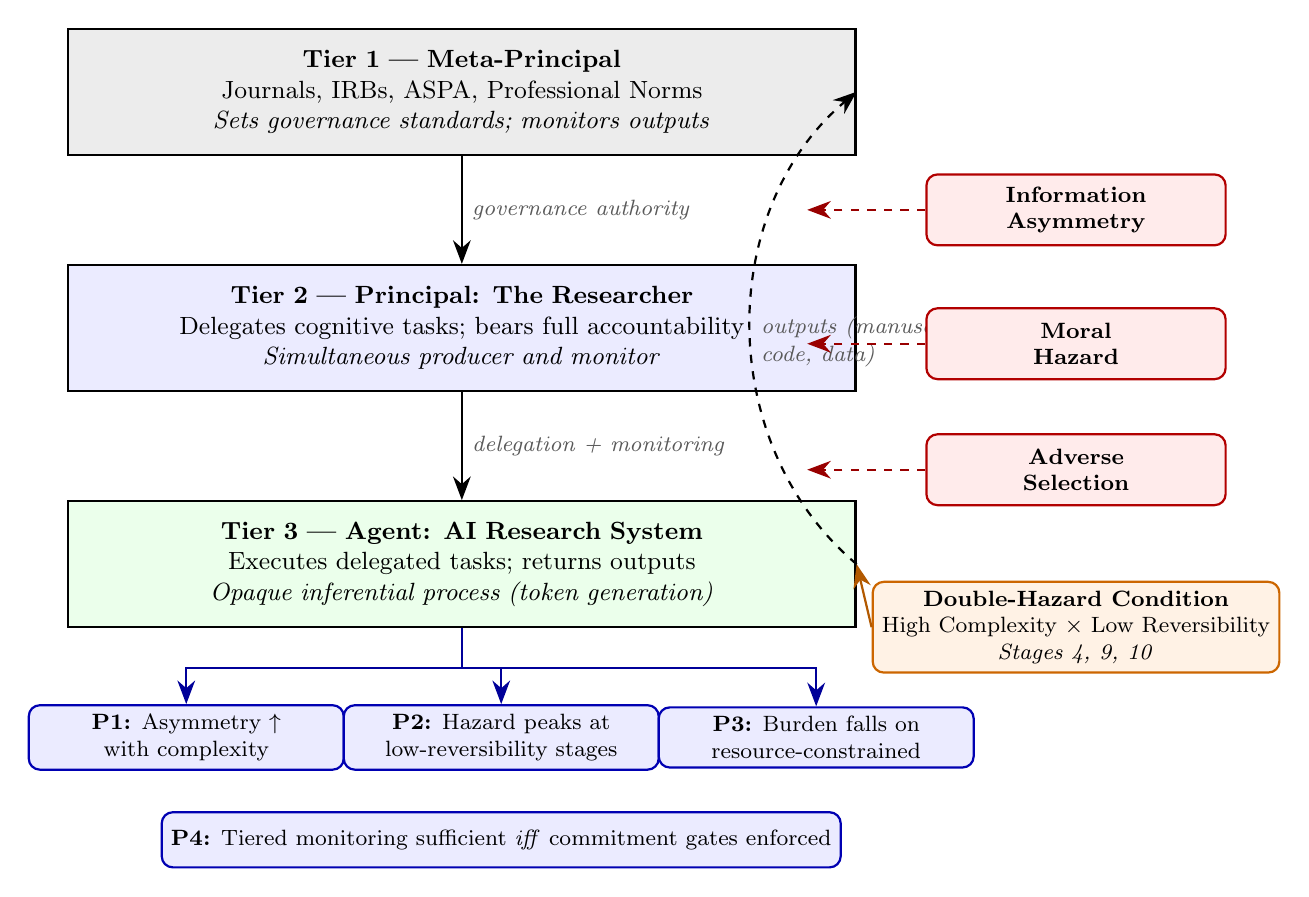
\begin{tikzpicture}[
  tier/.style={rectangle, draw=black, thick, minimum width=10cm, minimum height=1.6cm,
               text width=9.5cm, align=center, font=\small},
  arrow/.style={-{Stealth[length=3mm]}, thick},
  doublearrow/.style={{Stealth[length=3mm]}-{Stealth[length=3mm]}, thick},
  problem/.style={rectangle, rounded corners, draw=red!70!black, fill=red!8, thick,
                  minimum width=3.8cm, minimum height=0.9cm, align=center, font=\footnotesize},
  prop/.style={rectangle, rounded corners, draw=blue!70!black, fill=blue!8, thick,
               minimum width=4cm, minimum height=0.7cm, align=center, font=\footnotesize},
  label/.style={font=\footnotesize\itshape, text=gray!70!black}
]

% Tier 1: Meta-Principal
\node[tier, fill=gray!15] (meta) at (0,8)
  {\textbf{Tier 1 --- Meta-Principal} \\
   Journals, IRBs, ASPA, Professional Norms \\
   \textit{Sets governance standards; monitors outputs}};

% Tier 2: Principal
\node[tier, fill=blue!8] (principal) at (0,5)
  {\textbf{Tier 2 --- Principal: The Researcher} \\
   Delegates cognitive tasks; bears full accountability \\
   \textit{Simultaneous producer and monitor}};

% Tier 3: Agent
\node[tier, fill=green!8] (agent) at (0,2)
  {\textbf{Tier 3 --- Agent: AI Research System} \\
   Executes delegated tasks; returns outputs \\
   \textit{Opaque inferential process (token generation)}};

% Governance arrows
\draw[arrow] (meta.south) -- node[right, label] {governance authority} (principal.north);
\draw[arrow] (principal.south) -- node[right, label] {delegation + monitoring} (agent.north);
\draw[arrow, dashed] (agent.east) to[bend left=50] node[right, label] {outputs (manuscripts,} node[right, label, yshift=-0.35cm] {code, data)} (meta.east);

% Agency problems (right side)
\node[problem] (ia) at (7.8, 6.5) {\textbf{Information} \\ \textbf{Asymmetry}};
\node[problem] (mh) at (7.8, 4.8) {\textbf{Moral} \\ \textbf{Hazard}};
\node[problem] (as) at (7.8, 3.2) {\textbf{Adverse} \\ \textbf{Selection}};

\draw[arrow, red!60!black, dashed] (ia.west) -- +(-1.5,0);
\draw[arrow, red!60!black, dashed] (mh.west) -- +(-1.5,0);
\draw[arrow, red!60!black, dashed] (as.west) -- +(-1.5,0);

% Propositions (below)
\node[prop] (p1) at (-3.5, -0.2) {\textbf{P1:} Asymmetry $\uparrow$ \\ with complexity};
\node[prop] (p2) at (0.5, -0.2) {\textbf{P2:} Hazard peaks at \\ low-reversibility stages};
\node[prop] (p3) at (4.5, -0.2) {\textbf{P3:} Burden falls on \\ resource-constrained};
\node[prop, minimum width=6cm] (p4) at (0.5, -1.5) {\textbf{P4:} Tiered monitoring sufficient \textit{iff} commitment gates enforced};

\draw[arrow, blue!60!black] (agent.south) -- ++(0,-0.5) -| (p1.north);
\draw[arrow, blue!60!black] (agent.south) -- ++(0,-0.5) -| (p2.north);
\draw[arrow, blue!60!black] (agent.south) -- ++(0,-0.5) -| (p3.north);

% Double-hazard annotation
\node[rectangle, rounded corners, draw=orange!80!black, fill=orange!10, thick,
      minimum width=4.5cm, align=center, font=\footnotesize] (dh) at (7.8, 1.2)
  {\textbf{Double-Hazard Condition} \\
   High Complexity $\times$ Low Reversibility \\
   \textit{Stages 4, 9, 10}};

\draw[arrow, orange!70!black, thick] (dh.west) -- (agent.east);

\end{tikzpicture}
\caption{The Research-Agent Principal Hierarchy (RAPH): Theoretical Framework and Hypothesized Relations.
The three-tier governance architecture generates three agency problems (right), which yield four testable
propositions (bottom). The double-hazard condition (orange box) emerges at the intersection of P1 and P2.
Dashed output line shows the accountability path from agent through researcher to field institutions.}
\label{fig:framework}
\end{figure}

\newpage
\begin{figure}[p]
\centering
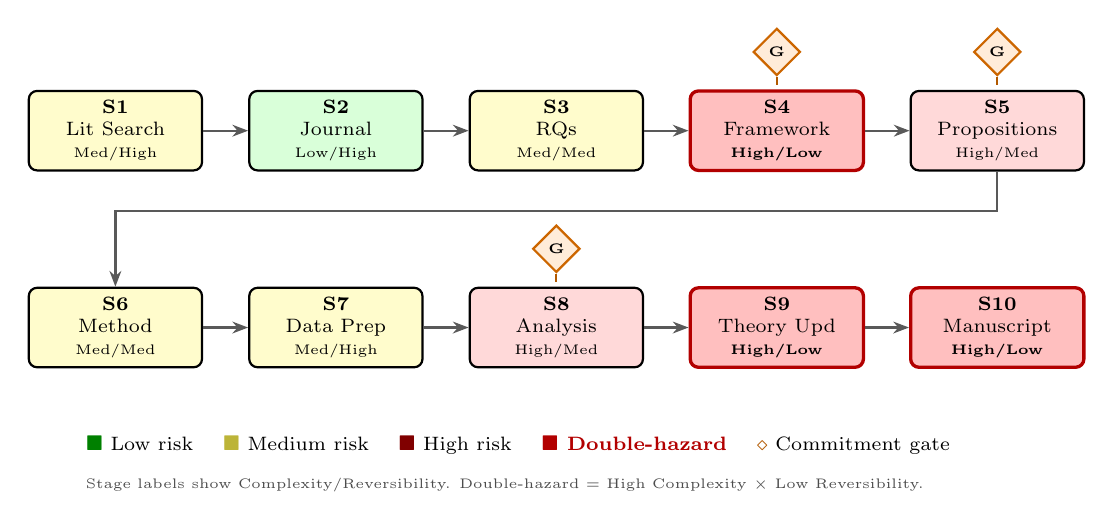
\begin{tikzpicture}[
  stage/.style={rectangle, rounded corners=3pt, draw=black, thick,
                minimum width=2.2cm, minimum height=0.8cm, align=center, font=\scriptsize},
  low/.style={fill=green!15},
  med/.style={fill=yellow!20},
  high/.style={fill=red!15},
  dh/.style={fill=red!25, draw=red!70!black, very thick},
  flowarrow/.style={-{Stealth[length=2mm]}, thick, gray!70!black},
  gate/.style={diamond, draw=orange!80!black, fill=orange!15, thick,
               minimum width=0.6cm, minimum height=0.6cm, inner sep=1pt, font=\tiny},
  bracelab/.style={font=\scriptsize\itshape, text=gray!60!black}
]

% Row 1: Stages 1-5
\node[stage, med] (s1) at (0,0) {\textbf{S1} \\ Lit Search \\ \tiny Med/High};
\node[stage, low] (s2) at (2.8,0) {\textbf{S2} \\ Journal \\ \tiny Low/High};
\node[stage, med] (s3) at (5.6,0) {\textbf{S3} \\ RQs \\ \tiny Med/Med};
\node[stage, dh]  (s4) at (8.4,0) {\textbf{S4} \\ Framework \\ \tiny \textbf{High/Low}};
\node[stage, high] (s5) at (11.2,0) {\textbf{S5} \\ Propositions \\ \tiny High/Med};

% Row 2: Stages 6-10
\node[stage, med] (s6) at (0,-2.5) {\textbf{S6} \\ Method \\ \tiny Med/Med};
\node[stage, med] (s7) at (2.8,-2.5) {\textbf{S7} \\ Data Prep \\ \tiny Med/High};
\node[stage, high] (s8) at (5.6,-2.5) {\textbf{S8} \\ Analysis \\ \tiny High/Med};
\node[stage, dh]  (s9) at (8.4,-2.5) {\textbf{S9} \\ Theory Upd \\ \tiny \textbf{High/Low}};
\node[stage, dh]  (s10) at (11.2,-2.5) {\textbf{S10} \\ Manuscript \\ \tiny \textbf{High/Low}};

% Flow arrows
\draw[flowarrow] (s1) -- (s2);
\draw[flowarrow] (s2) -- (s3);
\draw[flowarrow] (s3) -- (s4);
\draw[flowarrow] (s4) -- (s5);
\draw[flowarrow] (s5.south) -- ++(0,-0.5) -| (s6.north);
\draw[flowarrow] (s6) -- (s7);
\draw[flowarrow] (s7) -- (s8);
\draw[flowarrow] (s8) -- (s9);
\draw[flowarrow] (s9) -- (s10);

% Commitment gates
\node[gate] (g4) at (8.4, 1.0) {\textbf{G}};
\node[gate] (g5) at (11.2, 1.0) {\textbf{G}};
\node[gate] (g8) at (5.6, -1.5) {\textbf{G}};

\draw[orange!70!black, thick, dashed] (g4) -- (s4);
\draw[orange!70!black, thick, dashed] (g5) -- (s5);
\draw[orange!70!black, thick, dashed] (g8) -- (s8);

% Legend
\node[font=\scriptsize, anchor=west] at (-0.5, -4.0)
  {\textcolor{green!50!black}{$\blacksquare$} Low risk \quad
   \textcolor{yellow!70!black}{$\blacksquare$} Medium risk \quad
   \textcolor{red!50!black}{$\blacksquare$} High risk \quad
   \textcolor{red!70!black}{$\blacksquare$\textbf{ Double-hazard}} \quad
   \textcolor{orange!70!black}{$\diamond$} Commitment gate};

% Brace: Complexity/Reversibility label
\node[font=\tiny, text=gray!60!black, anchor=west] at (-0.5, -4.5)
  {Stage labels show Complexity/Reversibility. Double-hazard = High Complexity $\times$ Low Reversibility.};

\end{tikzpicture}
\caption{The 10-Stage AI-Assisted Research Pipeline with Risk Classification and Commitment Gates.
Red-bordered stages (4, 9, 10) are double-hazard junctures requiring structurally enforced commitment
gates (orange diamonds). Color intensity reflects combined agency risk (complexity $\times$ reversibility).}
\label{fig:researchflow}
\end{figure}

\newpage
\begin{figure}[p]
\centering
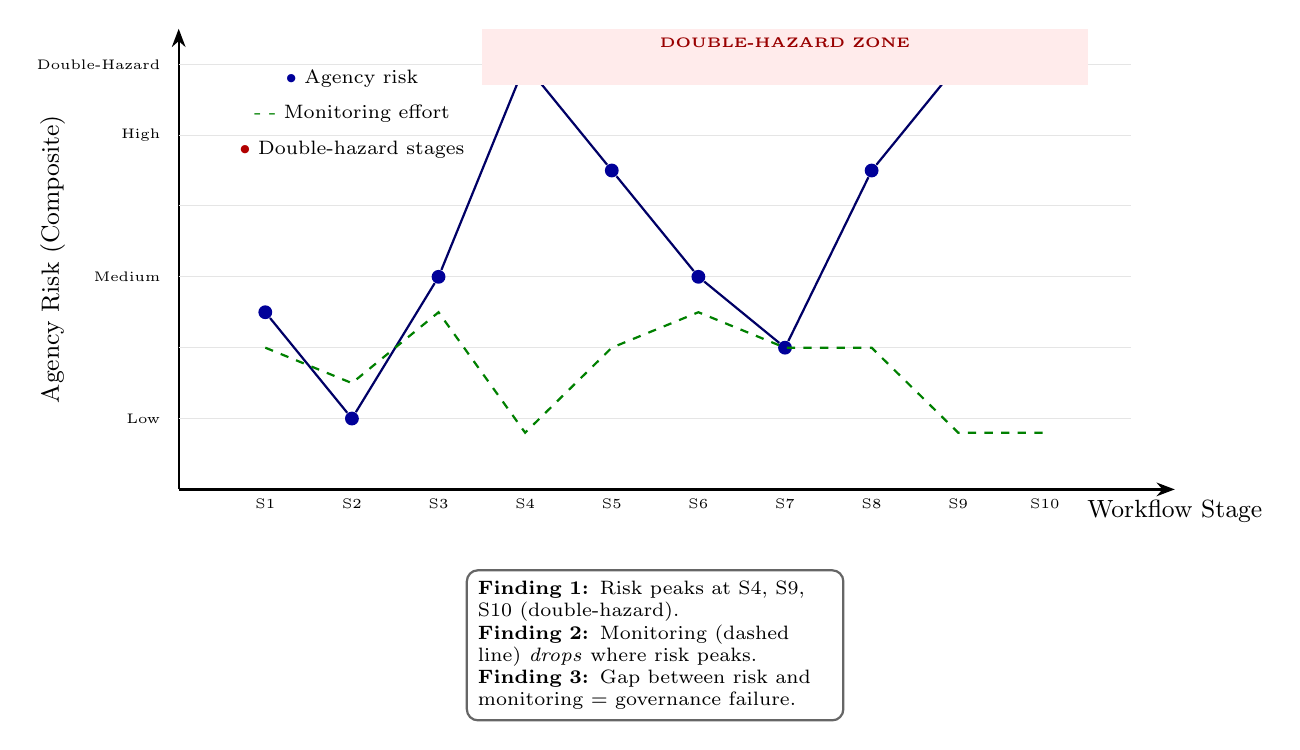
\begin{tikzpicture}[
  xscale=1.1, yscale=0.9,
  dot/.style={circle, fill=blue!60!black, minimum size=5pt, inner sep=0pt},
  dhdot/.style={circle, fill=red!70!black, minimum size=7pt, inner sep=0pt},
  findbox/.style={rectangle, rounded corners, draw=black!60, fill=white, thick,
                  text width=4.5cm, align=left, font=\scriptsize, inner sep=4pt}
]

% Axes
\draw[-{Stealth}, thick] (0,0) -- (11.5,0) node[below, font=\small] {Workflow Stage};
\draw[-{Stealth}, thick] (0,0) -- (0,6.5);
\node[font=\small, rotate=90, anchor=south] at (-1.2, 3.25) {Agency Risk (Composite)};

% Grid lines
\foreach \y in {1,2,3,4,5,6} {
  \draw[gray!20] (0,\y) -- (11,\y);
}

% Y-axis labels
\node[font=\tiny, anchor=east] at (-0.1, 1) {Low};
\node[font=\tiny, anchor=east] at (-0.1, 3) {Medium};
\node[font=\tiny, anchor=east] at (-0.1, 5) {High};
\node[font=\tiny, anchor=east] at (-0.1, 6) {Double-Hazard};

% Stage x-positions and risk values
% S1:2.5, S2:1, S3:3, S4:6, S5:4.5, S6:3, S7:2, S8:4.5, S9:6, S10:6
\node[font=\tiny, anchor=north] at (1,0) {S1};
\node[font=\tiny, anchor=north] at (2,0) {S2};
\node[font=\tiny, anchor=north] at (3,0) {S3};
\node[font=\tiny, anchor=north] at (4,0) {S4};
\node[font=\tiny, anchor=north] at (5,0) {S5};
\node[font=\tiny, anchor=north] at (6,0) {S6};
\node[font=\tiny, anchor=north] at (7,0) {S7};
\node[font=\tiny, anchor=north] at (8,0) {S8};
\node[font=\tiny, anchor=north] at (9,0) {S9};
\node[font=\tiny, anchor=north] at (10,0) {S10};

% Data points
\node[dot] (d1) at (1, 2.5) {};
\node[dot] (d2) at (2, 1) {};
\node[dot] (d3) at (3, 3) {};
\node[dhdot] (d4) at (4, 6) {};
\node[dot] (d5) at (5, 4.5) {};
\node[dot] (d6) at (6, 3) {};
\node[dot] (d7) at (7, 2) {};
\node[dot] (d8) at (8, 4.5) {};
\node[dhdot] (d9) at (9, 6) {};
\node[dhdot] (d10) at (10, 6) {};

% Connect dots
\draw[blue!40!black, thick] (d1) -- (d2) -- (d3) -- (d4) -- (d5) -- (d6) -- (d7) -- (d8) -- (d9) -- (d10);

% Double-hazard zone shading
\fill[red!8] (3.5, 5.7) rectangle (10.5, 6.5);
\node[font=\tiny\bfseries, text=red!60!black] at (7, 6.3) {DOUBLE-HAZARD ZONE};

% Monitoring level (dashed line)
\draw[green!50!black, thick, dashed]
  (1, 2) -- (2, 1.5) -- (3, 2.5) -- (4, 0.8) -- (5, 2) -- (6, 2.5) -- (7, 2) -- (8, 2) -- (9, 0.8) -- (10, 0.8);

% Key finding annotations
\node[findbox] at (5.5, -2.2)
  {\textbf{Finding 1:} Risk peaks at S4, S9, S10 (double-hazard). \\
   \textbf{Finding 2:} Monitoring (dashed line) \emph{drops} where risk peaks. \\
   \textbf{Finding 3:} Gap between risk and monitoring = governance failure.};

% Legend
\node[font=\scriptsize] at (2, 5.8)
  {\textcolor{blue!60!black}{$\bullet$} Agency risk};
\node[font=\scriptsize] at (2, 5.3)
  {\textcolor{green!50!black}{- -} Monitoring effort};
\node[font=\scriptsize] at (2, 4.8)
  {\textcolor{red!70!black}{$\bullet$} Double-hazard stages};

\end{tikzpicture}
\caption{Agency Risk versus Researcher Monitoring Effort across the 10-Stage Pipeline.
Composite agency risk (solid blue) peaks at double-hazard stages (S4, S9, S10), while researcher
monitoring effort (dashed green) drops at exactly those junctures --- the central governance failure
identified by the RAPH framework. The widening gap between risk and monitoring constitutes the
``moral hazard valley'' that structurally enforced commitment gates address.}
\label{fig:findings}
\end{figure}

\end{document}
